\documentclass{beamer}
\usetheme{CambridgeUS}

\setbeamertemplate{caption}[numbered]{}

\usepackage{enumitem}
\usepackage{tfrupee}
\usepackage{amsmath}
\usepackage{amssymb}
\usepackage{textcomp, gensymb}
\usepackage{graphicx}
\usepackage{txfonts}
                               
\providecommand{\pr}[1]{\ensuremath{\Pr\left(#1\right)}}
\providecommand{\mbf}{\mathbf}
\providecommand{\qfunc}[1]{\ensuremath{Q\left(#1\right)}}
\providecommand{\sbrak}[1]{\ensuremath{{}\left[#1\right]}}
\providecommand{\lsbrak}[1]{\ensuremath{{}\left[#1\right.}}
\providecommand{\rsbrak}[1]{\ensuremath{{}\left.#1\right]}}
\providecommand{\brak}[1]{\ensuremath{\left(#1\right)}}
\providecommand{\lbrak}[1]{\ensuremath{\left(#1\right.}}
\providecommand{\rbrak}[1]{\ensuremath{\left.#1\right)}}
\providecommand{\cbrak}[1]{\ensuremath{\left\{#1\right\}}}
\providecommand{\lcbrak}[1]{\ensuremath{\left\{#1\right.}}
\providecommand{\rcbrak}[1]{\ensuremath{\left.#1\right\}}}
\providecommand{\abs}[1]{\vert#1\vert}
\newcommand*{\permcomb}[4][0mu]{{{}^{#3}\mkern#1#2_{#4}}}
\newcommand*{\perm}[1][-3mu]{\permcomb[#1]{P}}
\newcommand*{\comb}[1][-1mu]{\permcomb[#1]{C}}

\newcounter{saveenumi}
\newcommand{\seti}{\setcounter{saveenumi}{\value{enumi}}}
\newcommand{\conti}{\setcounter{enumi}{\value{saveenumi}}}

\makeatletter
\newenvironment<>{proofs}[1][\proofname]{%
    \par
    \def\insertproofname{#1\@addpunct{.}}%
    \usebeamertemplate{proof begin}#2}
  {\usebeamertemplate{proof end}}
\makeatother

\title{Assignment 10}
\author{Kotikalapudi Karthik (CS21BTECH11030)}
\date{\today}
\logo{\large \LaTeX{}}


\begin{document}

% Title page frame
\begin{frame}
    \titlepage 
\end{frame}

% Remove logo from the next slides
\logo{}


% Outline frame
\begin{frame}{Outline}
    \tableofcontents
\end{frame}

%Question
\section{Question}
\begin{frame}{Question}
    \begin{block}{Probability, Random Variables and Stochastic Processes Chapter 2, Problem 2-25} 
        A train and a bus arrive at the station at random between $9$ A.M. and $10$ A.M. The train stops for 10 minutes and the bus for x minutes. Find x so that the probability that the bus and the train will meet equals $0.5$
    \end{block}
\end{frame}

%Solution
\section{Solution}
\begin{frame}{Solution}
\begin{block}{}
    Let's denote the random variable $X_1$ map to the set $\cbrak{0,1}$ where $X_1 = 0$ denote that bus and train don't meet and $X_1=1$ denote that they meet.
\end{block}
\begin{block}{}
    Let's denote the random variable $X_2$ map to the set $\cbrak{0,1}$ where $X_2 = 0$ denote that bus arrives first and $X_2=1$ denote that train arrives first.
\end{block}
\end{frame}

\begin{frame}{Graph description}
    Given, train stops for 10 mins and bus stops for $x$ minutes.\\
    Let's draw a graph with Arrival time of bus in mins on X-axis and Arrival time of train in mins on Y-axis.\\
    For the region in which bus and train meet(in blue color),\\
    $Y<X+x$(train should arrive within $x$ minutes after the bus) and
    $X<Y+10$(bus should arrive within 10 minutes after the train)
\end{frame}

\section{Graph}
\begin{frame}{Graph}
    \begin{figure}[!ht]
		\centering
		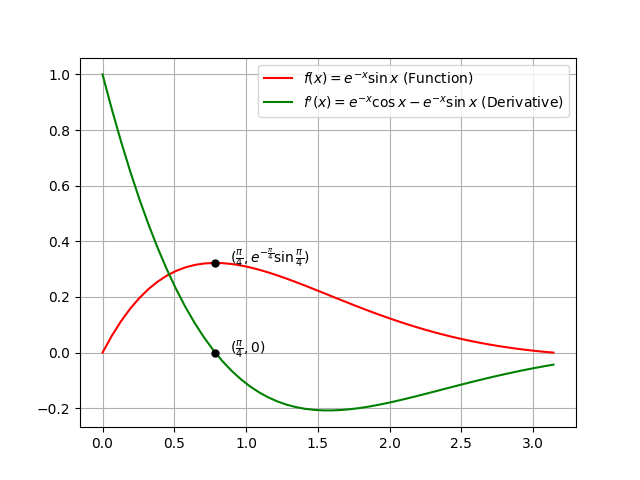
\includegraphics[width=\textwidth,height=5.5cm,keepaspectratio]{Figure_1.png}
		\caption{Arrival times of Bus and train}
		\label{fig:fig1}
	\end{figure}
\end{frame}

\section{Finding the value of x}
\begin{frame}{Finding the Value of x}
    \begin{align}
        \text{Given, }\frac{\pr{X_1=1}}{\Sigma^{1}_{i=0}\pr{X_1=i}} &= 0.5\\
        \implies \frac{\pr{X_1=0}}{\Sigma^{1}_{i=0}\pr{X_1=i}} &= 0.5
        \label{eq:eq-1}
    \end{align}
    Substituting the values from the Figure \eqref{fig:fig1} in equation \eqref{eq:eq-1},
    \begin{align}
        \frac{\frac{1}{2}\sbrak{\brak{60-x}^2+50\times50}}{60\times60} &= 0.5
        \\
        \implies \brak{60-x}^2+50\times50 &= 60\times60
        \\
        \implies \brak{60-x}^2 &= 1100
        \\
        \implies x &= 60 - 10\sqrt{11} \approx 26.83 \text{ mins}
    \end{align}
\end{frame}

\end{document}